The device is  assembled (as can be seein  in Figure \ref{fig:bat6:assembled})
and has  a functioning interface. Thanks  to our custom  PCB, we were  able to
make a very compact device (visible in Figure \ref{fig:bat6:internals}).  Most
sub circuits function  as intended (OLED, button, USB,  microchip), except for
the circuitry related to the buck  converter.  The front-end software has been
successfully brought to proof-of-concept stage  and is ready to be implemented
fully.

The  primary  thing   which  does  not  function  as  intended   is  the  buck
converter. We were however able to pinpoint  the likely cause of the issue and
are confident that  with more time and  a new hardware revision,  we could fix
this problem.

The next step would  now be to print a new PCB with  improvements based on our
simulations  from  section  \ref{sec:verification}  and  then  verify  correct
functionality of our device.

\begin{figure}[h!]
    \center
    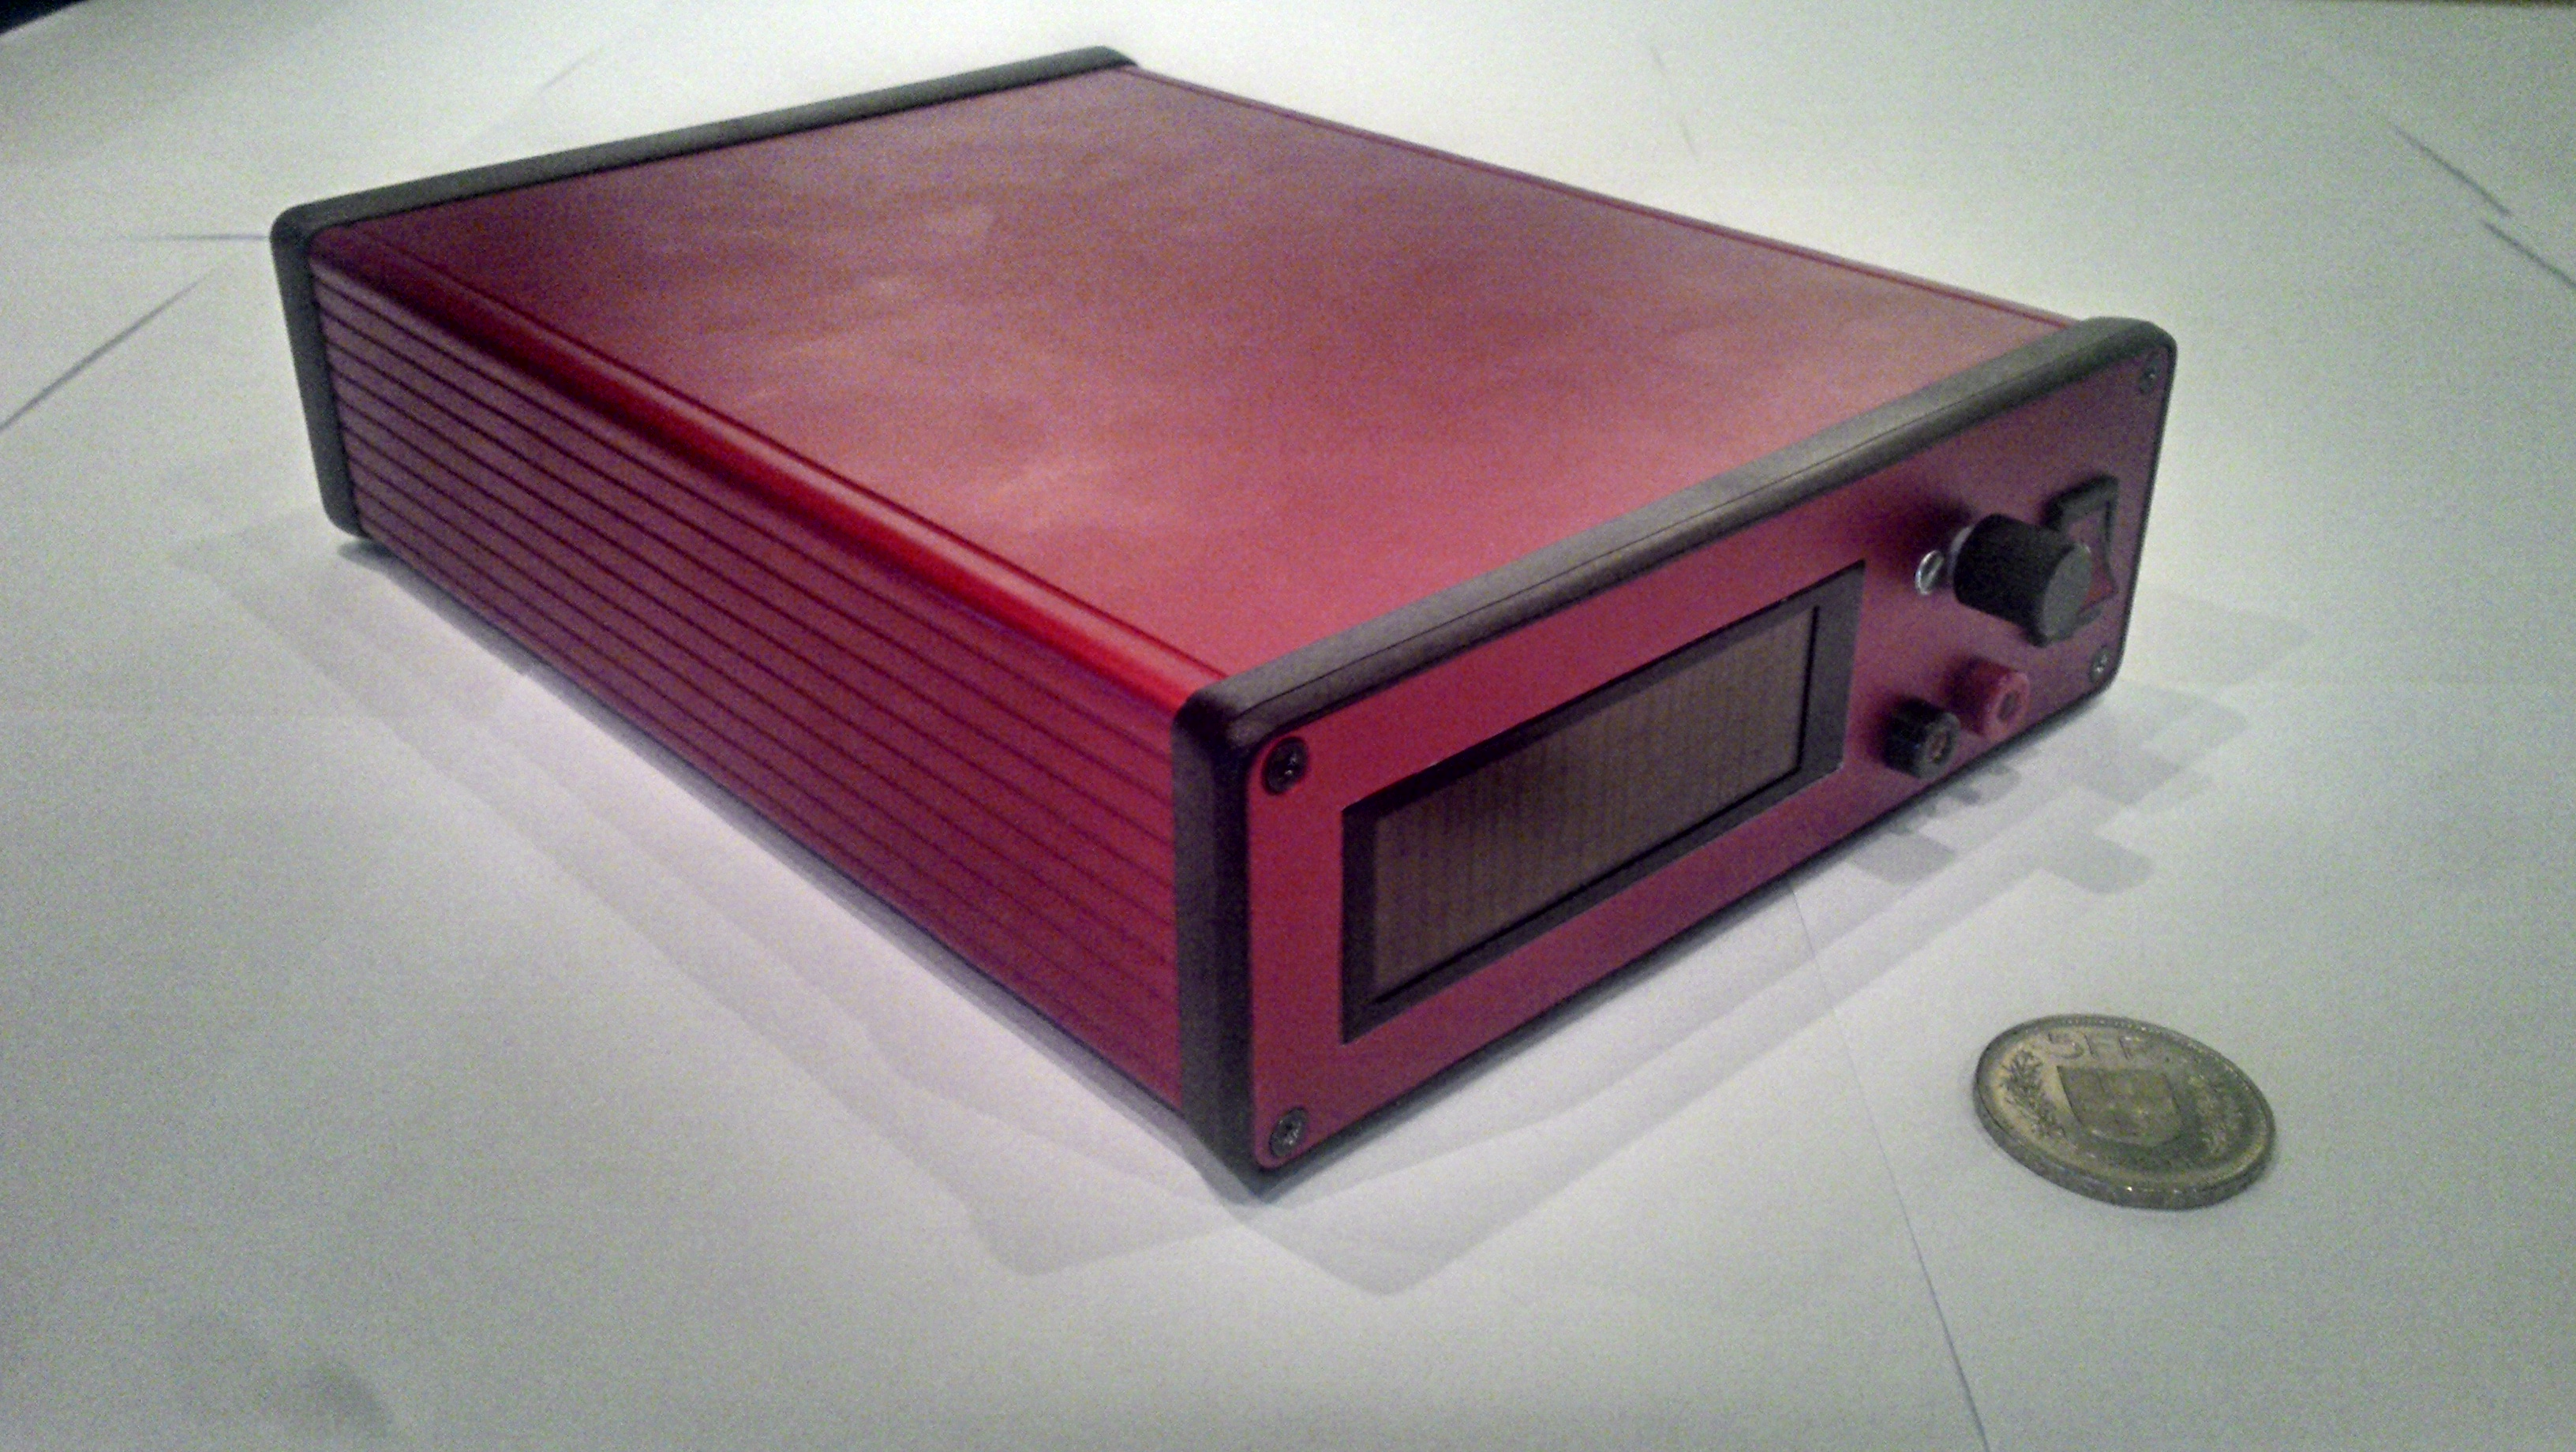
\includegraphics[width=.8\textwidth]{images/assembled.jpg}
    \caption{\emph{BAT6} assembled, 5 CHF coin for scale}
    \label{fig:bat6:assembled}
\end{figure}

\begin{figure}[h!]
    \center
    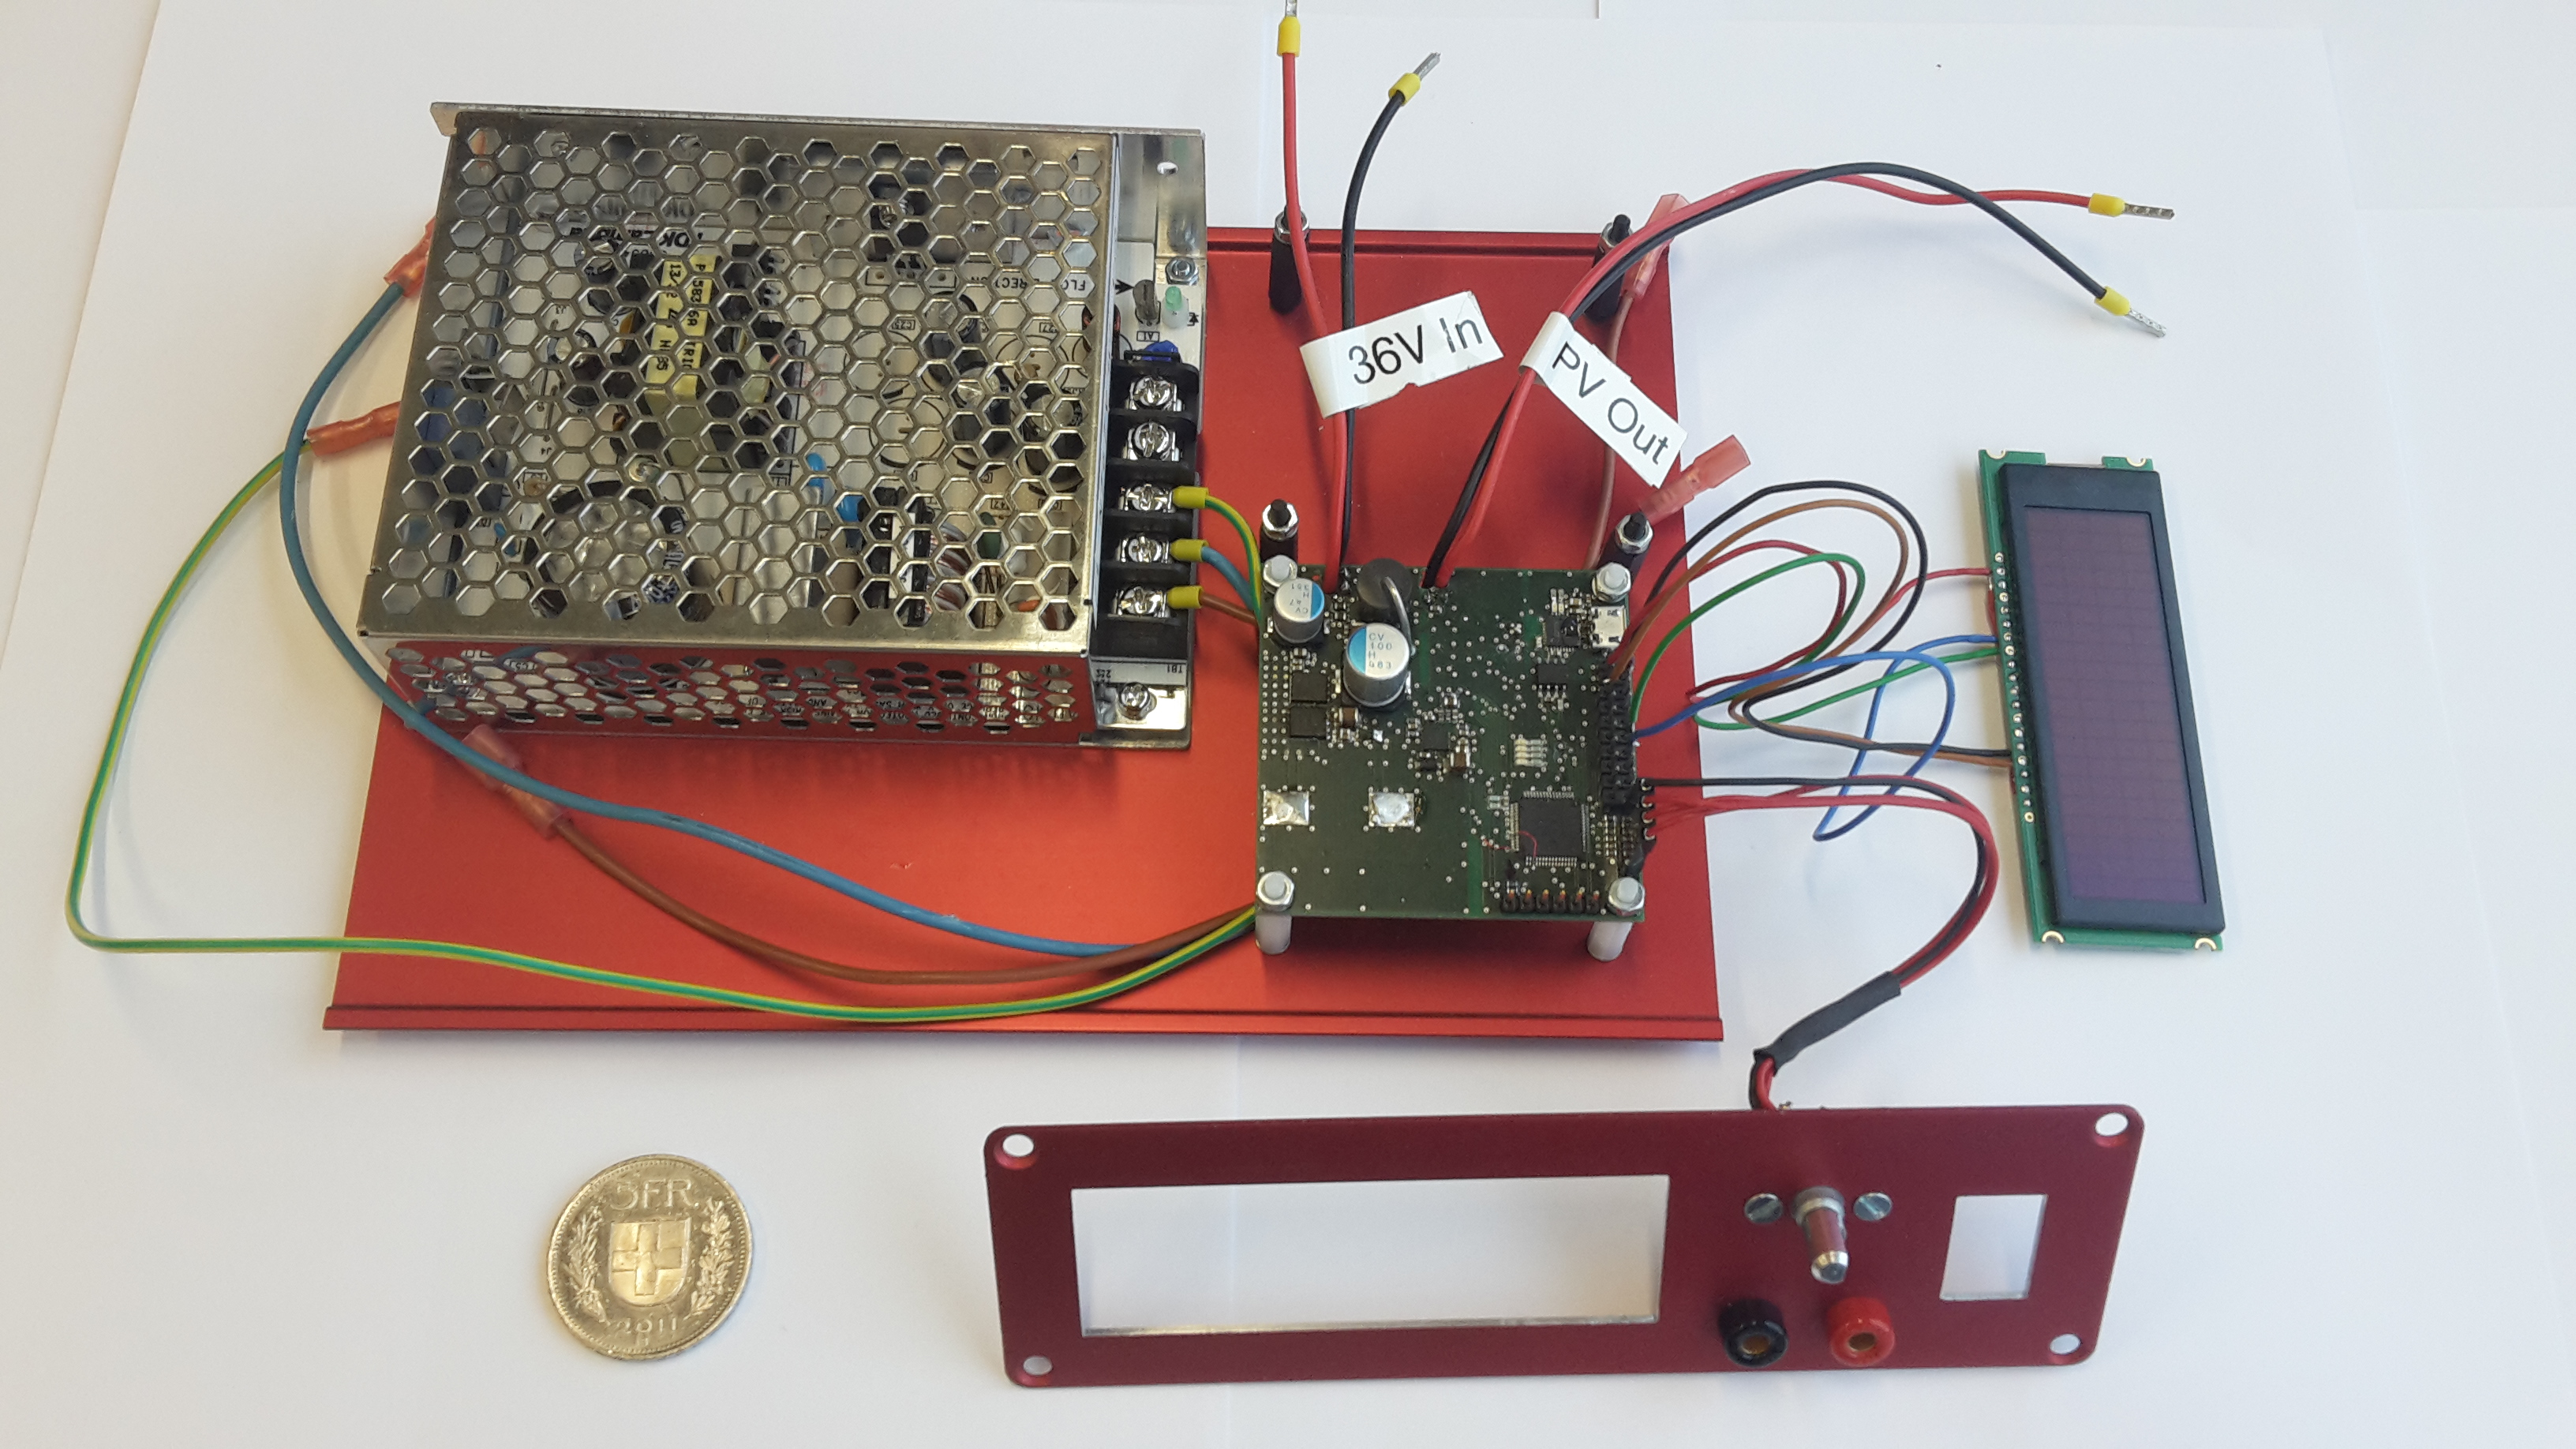
\includegraphics[width=.8\textwidth]{images/internals.jpg}
    \caption{\emph{BAT6}'s internals. Note the PCB's compact size. Most of the internal space is taken up by the power supply. 5 CHF coin for scale.}
    \label{fig:bat6:internals}
\end{figure}
